\documentclass[a4paper,11pt]{article}

\usepackage[utf8]{inputenc}
\usepackage[T1]{fontenc} % LY1 also works
\usepackage[margin=1in]{geometry}

%% Font settings suggested by fbb documentation.
\usepackage{textcomp} % to get the right copyright, etc.
\usepackage[lining,tabular]{fbb} % so math uses tabular lining figures
\usepackage[scaled=.95,type1]{cabin} % sans serif in style of Gill Sans
\usepackage[varqu,varl]{zi4}% inconsolata typewriter
\useosf % change normal text to use proportional oldstyle figures
%\usetosf would provide tabular oldstyle figures in text

\usepackage{microtype}
\usepackage{siunitx}
\DeclareSIUnit{\belmilliwatt}{Bm}
\DeclareSIUnit{\dBm}{\deci\belmilliwatt}
\sisetup{range-phrase=--, range-units=single, binary-units = true}
\usepackage{graphicx}
\usepackage{tikz}
\usepackage{svg}
%\usepackage{hyperref}
\usetikzlibrary{arrows, shadows}
\tikzset{%
  cascaded/.style = {%
    general shadow = {%
      shadow scale = 1,
      shadow xshift = -1ex,
      shadow yshift = 1ex,
      draw,
      thick,
      fill = white},
    general shadow = {%
      shadow scale = 1,
      shadow xshift = -.5ex,
      shadow yshift = .5ex,
      draw,
      thick,
      fill = white},
    fill = white, 
    draw,
    thick,
    minimum width = 1.5cm,
    minimum height = 2cm}}
    
\usepackage{enumitem}
\setitemize{noitemsep,topsep=0pt,parsep=0pt,partopsep=0pt}
\setlist{leftmargin=*}
\usepackage{listings}
\lstset{
	basicstyle=\ttfamily,
	frame=single,
	breaklines=true,
	morecomment=[l][\color{green}]{\#},
}
\usepackage[os=win]{menukeys}
\renewmenumacro{\keys}[+]{shadowedroundedkeys}

\usepackage{booktabs,caption}
\usepackage[flushleft]{threeparttable}
\newcolumntype{L}[1]{>{\raggedright\let\newline\\\arraybackslash\hspace{0pt}}m{#1}}
\newcolumntype{C}[1]{>{\centering\let\newline\\\arraybackslash\hspace{0pt}}m{#1}}
\newcolumntype{R}[1]{>{\raggedleft\let\newline\\\arraybackslash\hspace{0pt}}m{#1}}
\usepackage{tabularx} 

\usepackage{stackengine}
\usepackage{scalerel}
\usepackage{xcolor,mdframed}

\newcommand\danger[1][5ex]{%
  \renewcommand\stacktype{L}%
  \scaleto{\stackon[1.3pt]{\color{red}$\triangle$}{\tiny !}}{#1}%
}

\newenvironment{important}[1][]{%
   \begin{mdframed}[%
      backgroundcolor={red!15}, hidealllines=true,
      skipabove=0.7\baselineskip, skipbelow=0.7\baselineskip,
      splitbottomskip=2pt, splittopskip=4pt, #1]%
   \makebox[0pt]{% ignore the withd of !
      \smash{% ignor the height of !
         %\fontsize{32pt}{32pt}\selectfont% make the ! bigger
         \hspace*{-45pt}% move ! to the left
         \raisebox{-5pt}{% move ! up a little
            {\danger}% type the bold red !
         }%
      }%
   }%
}{\end{mdframed}}

\newcommand\info[1][5ex]{%
  \renewcommand\stacktype{L}%
  \scaleto{\stackon[1.2pt]{\color{blue}$\bigcirc$}{\raisebox{-1.5pt}{\small i}}}{#1}%
}

\newenvironment{information}[1][]{%
   \begin{mdframed}[%
      backgroundcolor={blue!15}, hidealllines=true,
      skipabove=0.7\baselineskip, skipbelow=0.7\baselineskip,
      splitbottomskip=2pt, splittopskip=4pt, #1]%
   \makebox[0pt]{% ignore the withd of !
      \smash{% ignor the height of !
         %\fontsize{32pt}{32pt}\selectfont% make the ! bigger
         \hspace*{-45pt}% move ! to the left
         \raisebox{-5pt}{% move ! up a little
            {\info}% type the bold red !
         }%
      }%
   }%
}{\end{mdframed}}

\usepackage{makecell}
\usepackage{hyperref}
\newcommand{\vna}{LibreVNA}

\newcommand{\screenshot}[2]{\begin{center}
\includegraphics[width=#1\textwidth]{Screenshots/#2}
\end{center}}

\title{\vna{} User Manual}
%\author{Jan Käberich (\url{j.kaeberich@gmx.de})}
\begin{document}
\maketitle

%\begin{abstract}
%The Testcard is a platform for the characterization of small energy sources. It is able to charge/discharge up to eight energy sources with a predefined pattern and record their voltages.
%\end{abstract}

\setcounter{tocdepth}{3}
\tableofcontents
\clearpage

%\section*{Nomenclature}
%
%\begin{description}
%\item[Testcard] Board with the hardware to characterize up to eight energy sources.
%\item[CLI] Command Line Interface. Program running on the computer which controls the testcard.
%\item[Channel] One of the eight measurement units on the testcard.
%\begin{description}
%\item[Voltage] Voltage of the energy source connected to the channel.
%\item[Current] Current flowing through the energy source connected to the channel. Defined as the current flowing from the energy source to the testcard, thus the source is discharged for positive and charged for negative values.
%\end{description}
%\item[Load] Application of a current at the channels for a specified timespan.
%\item[Measurement] Single measurement of channel voltages at a specified point in time.
%\item[Trace] Periodic measurement of channel voltages.
%\item[Sequence] A combination of loads, measurements and traces.
%\end{description}

\section{Overview}

\begin{tikzpicture}
\begin{scope}[xshift=1.5cm]
    \node[anchor=south west,inner sep=0] (image) at (0,0) {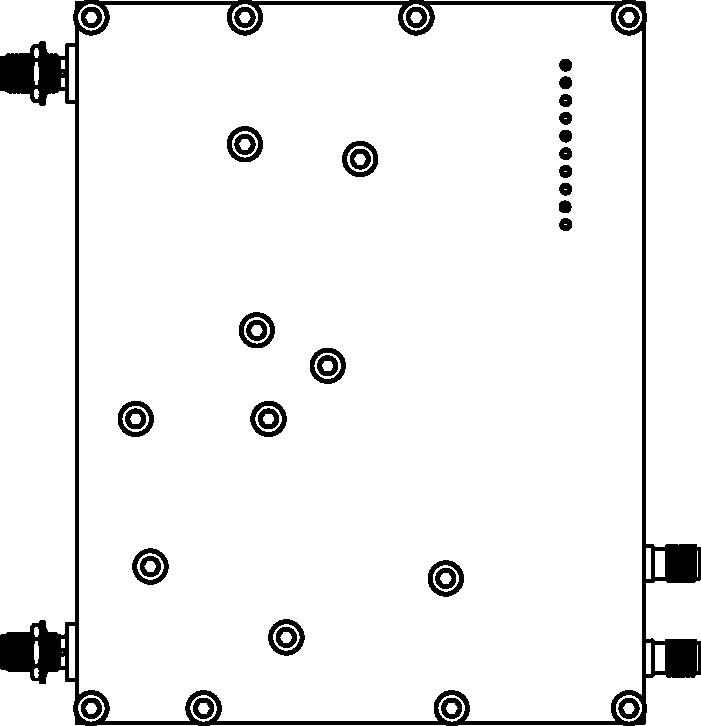
\includegraphics[width=0.76\textwidth]{TopDrawing.pdf}};
    \begin{scope}[x={(image.south east)},y={(image.north west)}]
		\node [anchor=south, align=center] (port1) at (0,1) {Port 1};
		\node [anchor=south, align=center] (port2) at (0,0.2) {Port 2};
		\node [anchor=west, align=center] (leds) at (1.05,0.8) {LEDs\\ \footnotesize Ready\\ \footnotesize Debug\\ \footnotesize Port1\\ \footnotesize Port2\\ \footnotesize Ext. Reference\\ \footnotesize Source unlocked\\ \footnotesize LO unlocked\\ \footnotesize FPGA unlocked\\ \footnotesize Booting\\ \footnotesize Power};
		\node [anchor=west, align=center] (power) at (1.05,0.5) {External Power \\ \footnotesize (optional)};
		\node [anchor=west, align=center] (usb) at (1.1,0.4) {USB};
		\node [anchor=west, align=center] (refout) at (1.1,0.2) {Reference\\Output};
		\node [anchor=west, align=center] (refin) at (1.1,0) {Reference \\Input};

        \draw [-*, ultra thick, gray] (port1) to[] (0.02,0.89);
        \draw [-*, ultra thick, gray] (port2) to[] (0.02,0.09);
        \draw [-*, ultra thick, gray] (leds) to[] (0.8,0.84);
        \draw [-*, ultra thick, gray] (power) to[] (0.91,0.55);
        \draw [-*, ultra thick, gray] (usb) to[] (0.91,0.5);
        \draw [-*, ultra thick, gray] (refout) to[] (0.97,0.23);
        \draw [-*, ultra thick, gray] (refin) to[] (0.97,0.1);
    \end{scope}
\end{scope}
\end{tikzpicture}%

\subsection{USB}
The \vna{} uses a USB-C connector as the power supply and for data transmission. The hardware supports the USB power delivery standard\footnote{Work in progress, the device will not negotiate USB-PD yet}, requires \SI{5}{\volt} and draws up to \SI{1.2}{\ampere} of current.

The implemented USB device is limited to USB 2.0 Fullspeed and data transmission will work with any USB 2.0 or 3.0 port (no USB-C required). However, the current consumption exceeds the specifications for USB 2.0 and 3.0 ports and the \vna{} may be unable to fully boot when no external power is applied USB host limits the current.
\subsection{External Power}
Input jack for external DC power (\SI{5}{\volt}, \SI{1.5}{\ampere}, positive center pin). If a power source is connected, no current is drawn from the USB port anymore.
\subsection{RF ports}
RF connector to connect the DUT. Both ports are identical and the device architecture support full S-Parameter measurements (S11, S21, S12 and S22).
\begin{important}
The RF ports have no input protection, do not apply a signal with more than +\SI{10}{\dBm} of power.
\end{important}
\subsection{LEDs}
Ten LEDs indicate the status:
\begin{description}
\item [Ready (green)] Indicates fully booted \vna{}, ready to take measurements
\item [Debug (green)] Not used at the moment
\item [Port 1 (green)] Active output signal on port 1
\item [Port 2 (green)] Active output signal on port 2
\item [Ext. Reference (green)] External reference in use
\item [Source unlocked (red)] The source PLL failed to lock (it may turn on briefly during a sweep, this is not a problem)
\item [LO unlocked (red)] The 1.LO PLL failed to lock (it may turn on briefly during a sweep, this is not a problem)
\item [FPGA unlocked (red)] The FPGA clock PLL failed to lock
\item [Booting (red)] Indicates boot process, also used for error codes
\item [Power (green)] USB power valid
\end{description}
\subsection{Reference Output}
Optional reference output port (user selectable \SI{10}{\mega\hertz} or \SI{100}{\mega\hertz}). The output power is approximately +\SI{3}{\dBm}.
\subsection{Reference Input}
High impedance reference input port. When applying a \SI{10}{\mega\hertz} input signal, it can be used to overwrite the internal TCXO.
\begin{information}
Due to the high impedance input, the external input may detect a valid signal when picking up external radiation. If this is a problem, either terminate the reference input connector or disable automatic reference switching.
\end{information}

\section{Getting started}
\begin{enumerate}
\item Connect the \vna{} to a computer using the USB port. After a couple of seconds, only the "Power" and "Ready" LEDs should stay on. If the "Ready" LED does not turn on or the "Booting" LED indicates an error code, there is a problem und the device will not function properly. See section~\ref{troubleshooting} for possible solutions.
\item Start the PC application to connect to the \vna{}. The window should look similar to this:
\makebox[\textwidth][c]{
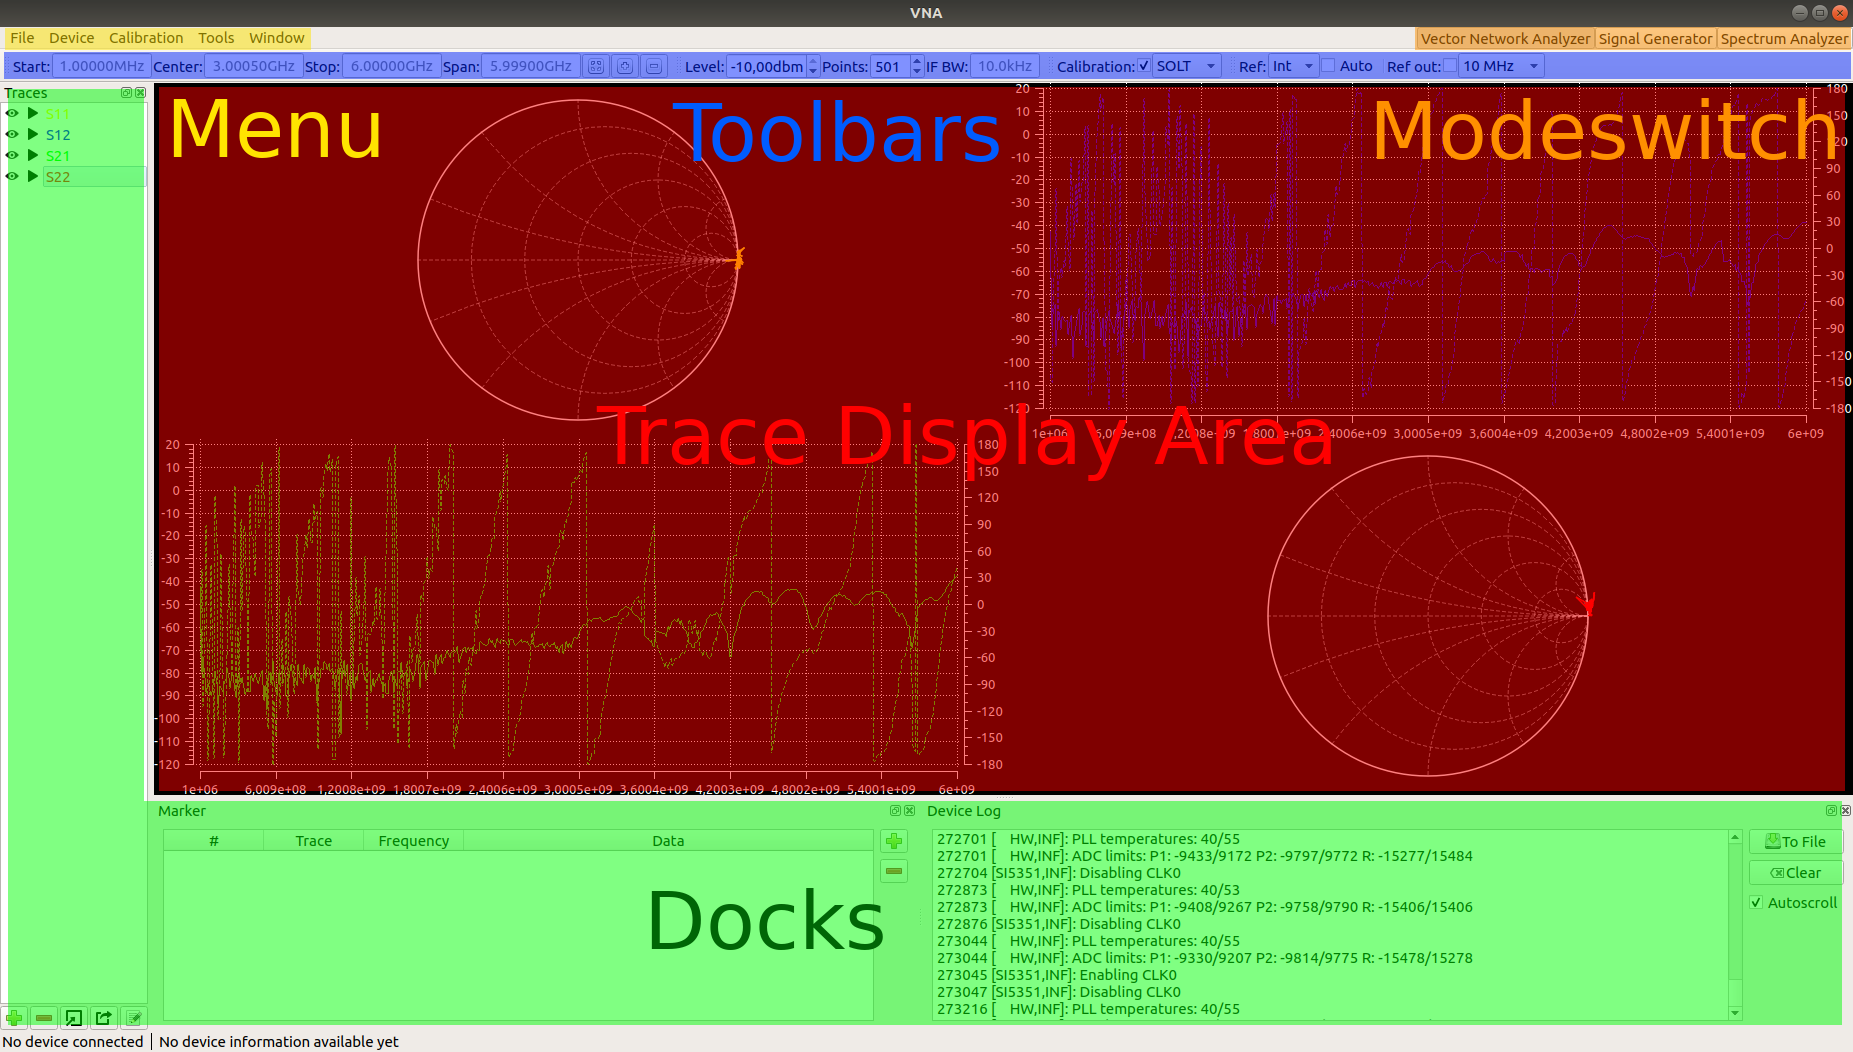
\includegraphics[width=\textwidth]{Screenshots/ApplicationOverview.png}
}
\end{enumerate}
\subsection{GUI element types}
The \vna{} application is made up of six areas containing different types of control:
\begin{itemize}
\item The \textbf{Trace Display Area} shows the measured data in various diagrams.
\item The \textbf{Toolbars} provide access to commonly used device settings. They can be rearranged or disabled (see section~\ref{menu:window}).
\item The \textbf{Menu} at the top left handles less common settings or more complex actions (often with additional popup windows).
\item The \textbf{Docks} mostly provide access to display related settings such as traces and markers. They can be rearranged or disabled (see section~\ref{menu:window}).
\item The \textbf{Statusbar} at the bottom show some basic informations about the connected device. If error conditions (e.g. ADC overload) are present, they are indicated at the bottom right corner.
\item The \textbf{Modeswitch} at the top right allows changing the \vna{} operating mode. Although it is primarily designed as a vector network analyzer, the hardware architecture allow some other operating modes with certain limitations.
\end{itemize}
Depending on the current operating mode, the available toolbars, docks and menu entries change. It is also possible to rearrange the docks and toolbars.

\subsection{Common GUI elements}
Certain control elements are always available, regardless of the selected mode. They control settings of the \vna{} that are not specific to any of the operating modes.

\paragraph{Entering values}\hfill\newline
Most entry fields support SI prefixes. To set a new value, type in the number followed by an SI prefix (e.g. to set \SI{3.2}{\giga\hertz} press \keys{3},\keys{.},\keys{2},\keys{\shift+G}). The accepted prefixes vary depending on the input (e.g. pico is a valid prefix for a capacitance while it will not be accepted for a frequency). 

\subsubsection{Reference Toolbar}
The reference toolbar controls the external reference output as well as the input.
\screenshot{0.5}{ToolbarReference.png}
The reference can be set to "Int" (internal TCXO), "Ext" (external \SI{10}{\mega\hertz} signal) or to automatic mode. In automatic mode, the reference will switch to the external input when a signal is detected, otherwise it will use the internal TCXO.

The external reference output may either be disabled or set to \SI{10}{\mega\hertz} or \SI{100}{\mega\hertz}.

\subsubsection{Device Log Dock}
This dock shows the debug output of the \vna{} (the same messages as on the internal UART port). It may help to identify problems, otherwise it is not required for operation.
\screenshot{1.0}{DockDeviceLog.png}

\subsubsection{File Menu}
Changing the default setup of the application can require a lot of configuration, especially if some of the more complicated math or de-embedding options are used. To simplify this process, setup-files can be saved and opened, which perform these steps automatically. A setup file contains all settings and configuration of these elements:
\begin{itemize}
\item Traces (Name, Color, Parameters, ...)
\item Math operations applied to the traces
\item Markers
\item De-embedding options
\item Graph setup and enabled traces
\end{itemize}
\begin{important}
If any part of the setup references another file (e.i. a trace imported from a touchstone file), only the filename is saved. Opening a setup file after moving/deleting any of the referenced files will result in missing data. 
\end{important}

\subsubsection{Device Menu}
The device menu controls the connection state, allows low level hardware access and to perform firmware updates:
\begin{itemize}
\item \textbf{Update Device List:} Scans the USB port for connected devices. Clicking this action simply updates the list of devices, no connection is established.
\item \textbf{Connect to:} Select which \vna{} to connect to. Different devices are identified by their serial number.
\item \textbf{Disconnect:} Disconnect from the \vna{}.
\item \textbf{Manual Control:} Starts the manual control dialog in which all hardware settings are accessible (mostly used for testing purposes):
\screenshot{1.0}{DialogManualControl.png}
\item \textbf{Firmware Update:} Load a new microcontroller firmware and FPGA configuration into the \vna{}. Do not disconnect power while updating the firmware!
\screenshot{0.6}{DialogFirmwareUpdate.png}
\end{itemize}

\subsubsection{Window Menu}
\label{menu:window}
The window menu allows hiding not needed toolbars and docks. It also contains some application preferences.

\section{Vector Network Analyzer}
In this operating mode, the \vna{} takes S-parameter measurements. A source signal is generated and alternately applied to the RF ports. The incoming signal at both RF ports is measured, resulting in the four S-parameters S11 and S21 (when the source signal is routed to port 1) as well as S12 and S22 (when it is routed to port 2).

\subsection{Signal processing architecture}
\label{vna:dsp}
This section contains some details of the signal flow inside the \vna{}-Application. Knowledge of the signal flow is not required to operate the \vna{} but may help to understand certain features and limitations.
\tikzstyle{block} = [draw, rectangle, 
    minimum height=3em, minimum width=6em]
\tikzstyle{sum} = [draw, fill=blue!20, circle, node distance=1cm]
\tikzstyle{input} = [coordinate]
\tikzstyle{output} = [coordinate]
\tikzstyle{pinstyle} = [pin edge={to-,thin,black}]
\tikzset{%
  cascaded/.style = {%
    general shadow = {%
      shadow scale = 1,
      shadow xshift = -1ex,
      shadow yshift = 1ex,
      draw,
      %thick,
      fill = white,
      },
    general shadow = {%
      shadow scale = 1,
      shadow xshift = -.5ex,
      shadow yshift = .5ex,
      draw,
      %thick,
      fill = white,
      },
    fill = white, 
    draw,
    %thick,
    %minimum width = 1.5cm,
    %minimum height = 2.1cm
    }}

% The block diagram code is probably more verbose than necessary
\begin{center}
\begin{tikzpicture}[auto, node distance=2cm,>=latex']
    % We start by placing the blocks
	\node [block] (VNA) {VNA Hardware};
	\node [block, below of=VNA] (cal) {Calibration};
	\node [block, below of=cal] (deemb)  {De-embedding};
	\node [cascaded, block, below of=deemb, align=center, node distance=3cm, minimum height=2cm] (traces)  {Traces\\ \\ \\};
	\node [block, dashed, minimum width=4em, minimum height=2em, below of=traces, node distance=0.2cm] (math) {Math};
	\node [cascaded, block, node distance=3cm, below of=traces] (graphs)  {Graphs};


	\draw [->] (VNA) -- node {uncalibrated S parameter set (S11,S12,S21,S22) over USB} (cal);
	\draw [->] (cal) -- node {calibrated S parameter set (S11,S12,S21,S22)} (deemb);
	\draw [->] (deemb) -- node {individual S parameters} ([yshift=1ex]traces.north);
	\node [left of=traces, node distance=4cm](import){};
	\draw [->] (import) -- node {imported files} ([xshift=-1ex]traces.west);
	\node [right of=traces, node distance=6cm](export){};
	\draw [->] (traces.east) -- node {CSV/Touchstone export} (export);
	\draw [->] (traces) -- node {complex frequency/time domain data} ([yshift=1ex]graphs.north);
\end{tikzpicture}
\end{center}

The central element of the signal flow is the concept of \textbf{traces}. A trace is created from a single S parameter across frequency (either measured by the \vna{} or imported from an external file). Once the data is captured in a trace, optional math operations may be applied to it (e.g. performing a TDR to transform the data into the time domain) and the result of these operations are passed on to the graphs.

When capturing data from the \vna{}, additional operations take place before the data is fed to the traces. First, the \vna{} measures the four S parameters between its two ports. The raw measurements are transferred through USB. The first processing block is the calibration (see also section~\ref{vna:calibration}), followed by optional de-embedding procedures. After the de-embedding, the four S parameters are split into individual S parameters and the relevant traces are updated.

This concept has several consequences when using the \vna{}, some of which are:
\begin{itemize}
\item You can always take calibration measurements. No matter how the de-embedding or math operations in the traces are set up, they will never influence the calibration routine
\item A valid calibration is required before using de-embedding options (otherwise, most de-embedding options won't be able to work properly)
\item Applying a calibration or de-embedding to traces imported from files is not possible
\item Once the data arrives in the traces, the S parameters are no longer associated (e.g. there is no connection between S11 and S21 anymore. It is possible to "pause" the trace capturing S11 while S21 continues to get updated)
\end{itemize}

\subsection{Sweep Toolbar}
This toolbar sets the swept frequency range.
\screenshot{1.0}{ToolbarSweep.png}
The start/stop and center frequency as well as the span can be set directly.

Additionally, the sweep toolbar contains buttons for zooming in/out around the center frequency and a preset to set the sweep to the full frequency range.
\subsection{Acquisition Toolbar}
\screenshot{0.7}{ToolbarVNAAcquisition.png}
\begin{itemize}
\item \textbf{Level:} The amount of power used for stimulus generation. The dynamic range decreases when using smaller values. It is recommended to use the highest available settings when measuring passive networks. When measuring active devices (e.g. amplifiers), decrease the stimulus power in such a way that the input power into any port does not rise above \SI{-10}{\dBm} to stay within the linear range of the \vna.
\item \textbf{Points:} Amount of measurement points in one sweep. More points provide finer frequency resolution but also increase sweep time.
\item \textbf{IF BW:} Bandwidth of final IF measurement. Low bandwidths increase the sweep time but improve the noisefloor. At higher frequencies (roughly above \SI{3}{\giga\hertz}), the dynamic range is limited by the isolation between the ports and decreasing the IF bandwidth does not improve the noisefloor anymore.
\item \textbf{Averaging:} Moving average across multiple sweeps.
\end{itemize}

\subsection{Traces}
Adding/configuring traces is handled by the \textbf{Trace Dock} (by default on the left side): 
\screenshot{0.3}{TraceDock.png}
The list shows all available traces, by default the four S parameters S11, S12, S21 and S22. Different icons in front of the trace names indicate the state of the trace. Clicking on one of the icons toggles the state:
\begin{itemize}
\item \includesvg[height=8pt]{Screenshots/visible}/\includesvg[height=10pt]{Screenshots/invisible}: Enable/disable global visibility: Shows/hides the trace an all graphs it is enabled on.
\item \includesvg[height=8pt]{Screenshots/play}/\includesvg[height=8pt]{Screenshots/pause}: Play/pause. Only available when the trace is fed from live VNA data, not when it was created from a touchstone file. Pausing a trace freezes the current data, new measurements from the \vna{} will not update the trace.
\item \includesvg[height=8pt]{Screenshots/math_enabled}/\includesvg[height=10pt]{Screenshots/math_disabled}: Enable/disable math. Only available if at least one math operation is present.
\end{itemize}

Creating a new trace or double clicking on an existing trace opens the "edit trace" window:
\screenshot{1.0}{TraceEdit.png}
On the left side, additional trace parameters can be changed, while the right side of the window handles math operations that will be applied to the trace data. The available trace parameters are:
\begin{itemize}
\item \textbf{Name}
\item \textbf{Color}
\item \textbf{Velocity factor} (only relevant when transforming into the time domain)
\item \textbf{Data source} (Live Capture/From File):
\begin{itemize}
\item \textbf{Live Capture:} The trace is updated from the data measured by the \vna{}. Additional parameters are:
\begin{itemize}
\item \textbf{Type:} Overwrite/Max hold/Min hold
\item \textbf{Parameter:} The S parameter data used for this trace
\end{itemize}
\item \textbf{From File:} The trace data is created from a touchstone file. Additional parameters are:
\begin{itemize}
\item \textbf{Filename}
\item \textbf{Parameter:} Select which S parameter the trace should use (in case of multi-port touchstone file)
\end{itemize}
\end{itemize}
\end{itemize}

\subsubsection{Math operations}
\label{trace:math}
The "math operations" section on the right contains the additional calculations that are performed on the trace data before it is displayed. Initially, it contains only one line (representing the measured data). New operations can be created using the buttons on the right. Each math operation adds a new line to the list, consisting of three columns:
\begin{itemize}
\item \textbf{Status:} Visual indication whether the calculation succeeded. On warnings or errors, a mouse-over text gives a hint about the problem.
\item \textbf{Description:} Short description of the configured math operation. Double clicking will open an (operation dependent) editing dialog providing more details.
\item \textbf{Output Domain:} Domain (Time or Frequency) of the data after this math operation. Certain math operations can only be applied to time domain data, others only to frequency domain data. The output domain at the last line decides in which domain the trace is displayed on the graphs.
\end{itemize}

Populated with several math operations, the window could look like this:
\screenshot{1.0}{TraceMath.png}
In this example, time domain gating is performed:
\begin{itemize}
\item A median filter is applied to the data, smoothing the trace a little bit (not actually necessary for the time domain gating)
\item Next, a TDR transformation creates the time domain response of the measurement
\item The impulse response is truncated at and above \SI{1}{\meter} with a custom expression
\item At last the time domain response is transformed back into the frequency domain with a DFT
\end{itemize}

\subsection{Calibration}
\label{vna:calibration}
This section is about the VNA calibration which is used to remove the effect of connectors and cables (as well as imperfections from the \vna{} itself). For the amplitude calibration see section~\ref{amplitude:calibration}.

Some general knowledge about the different calibration types is assumed, this manual only explains how to use them with the \vna{}.
\subsubsection{Introduction}
This section contains some implementation details of the calibration. It can be skipped but understanding them can be helpful when using the calibration.

To apply a calibration three things are required:
\begin{enumerate}
\item \textbf{Calibration kit:} It contains the definition of the calibration standards. When the calibration error terms are calculated, these definitions are taken into account.
\item \textbf{Measurements:} Raw (uncorrected) measurements of the calibration standards. Depending on the type of desired calibration, different measurement are required.
\item \textbf{Calibration type:} The calibration type determines which errors are corrected by the calibration and how the error terms are derived from the measurements.
\end{enumerate}
For the most accurate results, the calibration should be performed with the same settings (span, number of points, stimulus level, ...) as the intended measurement. However, it is possible to change these settings after the calibration. The calibration will be interpolated/extrapolated when a different span is used.

\subsubsection{Types}
Several different calibration types are available:
\begin{center}
\begin{threeparttable}
\begin{tabularx}{\textwidth}{L{2cm}|X|L{3cm}}
    \toprule
    \textbf{Type} & \textbf{Applied corrections} & \makecell{\textbf{Required}\\ \textbf{measurements}}\\
     \hline
      Port 1   	&    Removes influences of cables and setup at port 1 only & \makecell{Port 1 open\\ Port 1 short\\ Port 1 load}\\ 
    \hline
      Port 2   	&    Removes influences of cables and setup at port 2 only & \makecell{Port 2 open\\ Port 2 short\\ Port 2 load}\\ 
    \hline
      SOLT   	&   Full two-port calibration, removes influences at both ports and also corrects transmission measurement & \makecell{Port 1 open\\ Port 1 short\\ Port 1 load\\ Port 2 open\\ Port 2 short\\ Port 2 load\\ Through\\ Isolation(optional)}\\ 
    \hline
      Normalize   &  Only corrects for losses and phaseshift in through measurements. While this is not as accurate as SOLT, it is useful e.g. when measuring only the frequency response of a filter because it requires far less calibration measurements.  & \makecell{Through}\\ 
    \hline
      TRL   	&   Full two-port calibration but with different (less accurately defined) standards than SOLT & \makecell{Port 1 open/short\\ Port 2 open/short\\Through\\ Line}\\ 
      \bottomrule
\end{tabularx}
\end{threeparttable}
\end{center}

\subsubsection{Calibration Kit}
The calibration kit contains the calibration standard definitions used in the calibration. It can be edited through the menu: \menu[,]{Calibration,Edit Calibration Kit}

The calibration kit coefficients are split into two tabs, one for the SOLT standards and one for the TRL standards. If a calibration kit is saved, all standard definitions (SOLT and TRL) are stored, regardless of which tab is currently active. The type of calibration selects which standard definitions are used in the actual calibration.
\screenshot{1.0}{CalKitSolt.png}
\screenshot{1.0}{CalKitTRL.png}

SOLT standards can either be specified by parameters (preferred way, valid for all frequencies) or by providing measurement data of the standard, here shown as an example with the open standard:
\screenshot{0.3}{CalKitOpenMeasurement.png}
A touchstone file with the measurements is required. If the file contains data from more ports than required (for open, short and load 1-port measurements are needed, for the through 2-port measurements), the correct port(s) has to be selected. If any standard is defined by a measurement, the usable frequency range of the calibration kit is limited to the smallest common range of all measurement.
\paragraph{Example:} The open standard is defined by a measurement file containing data from \SIrange{10}{500}{\mega\hertz}. The load standard is defined by a measurement file containing data from \SIrange{50}{800}{\mega\hertz}. In this case the calibration kit can only be used in the range of \SIrange{50}{500}{\mega\hertz}.
\begin{important}
When saving the calibration kit, only the (relative) filenames of any used measurements are saved. For future use, the measurement files have to be kept in the same folder relative to the calibration kit file.
\end{important}

\subsubsection{Measurements}
\label{vna:cal:meas}
The calibration measurements can be found in \menu[,]{Calibration,Calibration Measurements}. It contains all possible measurements, regardless of the currently active calibration:
\screenshot{1.0}{CalibrationMeasurements.png}
To take a measurement, select the corresponding line and press \keys{Measure}.
\begin{information}
All measurements required by a calibration type must have the same start and stop frequencies as well as number of points. Do not change the span inbetween measurements.
\end{information}

\subsubsection{Enabling a calibration}
Either select the desired calibration type in the calibration menu or choose it in the calibration toolbar and enable the checkbox. If all required measurements have already been taken, the calibration is activated immediately. If some measurements are missing or have been taken with different span settings, applying the calibration is not possible. In that case, the calibration measurement dialog (see section~\ref{vna:cal:meas}) opens, this time only showing the necessary measurements required for the selected calibration type.

\paragraph{Example:} After starting the application, the following steps are necessary to perform a SOLT calibration.
\begin{enumerate}
\item Edit the calibration kit to match the standards used in the measurements or open a saved calibration kit file.
\item Change the span and acquisition settings to match the intended measurement. At this point no calibration is active yet, the measured data (here with both port directly connected) is inaccurate:
\screenshot{1.0}{VNAUncalibratedThrough.png}
\item Select \menu[,]{Calibration,Calibration Measurements} and take the required measurements. In this case, the measurement "Isolation" (optional for SOLT) has not been taken, as well as the "Line" measurement (not required for SOLT)
\screenshot{1.0}{CalibrationMeasurementsSOLT.png}
\item Close the "Calibration Measurements" window and activate the SOLT calibration by selecting \menu[,]{Calibration,SOLT}:
\screenshot{0.3}{MenuActivateSOLT.png}
Alternatively, the calibration can be activated by choosing "SOLT" in the toolbar and enabling the calibration checkbox:
\screenshot{0.3}{ToolbarActivateSOLT.png}
\item The calibration is active and connecting both ports directly results in a corrected measurement:
\screenshot{1.0}{VNACalibratedThrough.png}
\end{enumerate}

\subsubsection{Saving/Loading}
Once a calibration is active, it can be saved by selecting \menu[,]{Calibration,Save}. All raw measurements are saved together with the calibration type and the calibration kit (saved in an additional file with same filename as the calibration).

Similarly, a saved calibration can be opened by selecting \menu[,]{Calibration,Load}. It is applied immediately after opening.

\subsubsection{Assigning a default calibration to a device}
Once a calibration has been saved, it can be selected as the default calibration for a specific device. To do so, first connect to the device and then select \menu[,]{Device,Default Calibration,Assign...}. Once a default calibration has been assigned, it will automatically be opened and applied every time the application connects to that specific device.

\subsubsection{Viewing error terms/calibration measurements}
The error terms calculated from the calibration measurements as well as the raw measurements used to derive these error terms can be imported by selecting \menu[,]{Calibration,Import error terms as traces} or \menu[,]{Calibration,Import measurements as traces}. This feature is mostly intended to debug calibration problems and is not normally required. The nomenclature follows \href{https://www.rfmentor.com/sites/default/files/NA_Error_Models_and_Cal_Methods.pdf}{"Network Analyzer Error Models and Calibration Methods"} by Doug Rytting.

\subsection{De-embedding}
The de-embedding options are available under \menu[,]{Tools,De-embedding}. The GUI works similar to the math operations for traces (see section~\ref{trace:math}) but the de-embedding is performed before the data reaches the traces (compare with section~\ref{vna:dsp}).
\screenshot{0.8}{Deembedding.png}

Just like with the math operations, a list shows the de-embedding options. Once a new option is added (or is double clicked) a window opens which allows to configure the option. Depending on the de-embedding option, there might be some user adjustable parameters (e.g. the length and attenuation of a port extension) or the option needs a measurement from the \vna{} to calculate the de-embedding parameters (e.g. take a measurement to automatically measure the port extension length). If a measurement is required at any point, a new window opens with two choices to provide the measurement data:
\screenshot{0.9}{DeembeddingMeas.png}
The first possibility is to click the measure button (with the \vna{} connected) which starts a new measurement. The \vna{} connections must have been setup properly before (e.g. in the case of the port extension: extension cable connected and terminated either into an open or short. The exact setup depends on the de-embedding option). The other possibilty is to provide the measurement by using traces. This is useful if the same measurement has already been taken but the physical setup has changed since then. Select the correct traces for all required S parameters and click the "OK" button.

\section{Signal Generator}
In the signal generator mode, measurements are stopped and the \vna{} only outputs a CW signal.
\screenshot{0.8}{Signalgenerator.png}
The hardware is not optimized for signal generation which means that the output level is not very accurate, especially at higher frequencies (also see section~\ref{amplitude:calibration}). Also, the signal will contain higher levels of harmonics than one would normally expect from a signal generator.
\section{Spectrum Analyzer}
Although the \vna{} hardware is not designed to be used as a spectrum analyzer, the general hardware architecture of a spectrum analyzer is similar enough to that of a VNA to implement basic two-channel spectrum measurements. This is in no way on the same performance level as a dedicated spectrum analyzer but for simple measurements it might suffice if no other equipment is available. The main differences to a real spectrum analyzer are:
\begin{itemize}
\item \textbf{No input attenuator or pre-amplifier:} This means that the measurement range is essentially fixed to approximately \SI{-110}{\dBm} to \SI{-10}{\dBm}.
\item \textbf{No amplitude calibration:} The displayed signal level is not very accurate, especially at higher frequencies (also see section~\ref{amplitude:calibration}).
\item \textbf{No image rejection filters:} This is probably the most severe limitation, because it means that for every real signal several other signals will show up in the spectrum that are not actually present at the input. Most of the images can be filtered out by signal identification but some will remain (at lower amplitude) in the reported data.
\item \textbf{Highest resolution bandwidth is quite low:} The sweep speed is too slow to cover the complete frequency range of \SI{1}{\mega\hertz} to \SI{6}{\giga\hertz} in an acceptable time.
\end{itemize}

Most control elements (Frequencies, Span, Traces, Marker, ...) are indentical to the vector network analyzer mode.
\subsection{Acquisition Toolbar}
\screenshot{0.7}{ToolbarSAAcquisition.png}
\begin{itemize}
\item \textbf{RBW:} Resolution bandwidth. Lower values allow differentiating between signals at closer frequencies. Lower values also result in a reduced noisefloor but significantly increase sweep time.

For low RBWs, a faster DFT acquisition method is available. Instead of tuning the LOs to look at each frequency point by itself, several points can be measured at once by performing a DFT of the final IF. Due to limitations in the hardware and the available processing power, the DFT is limited to 96 points and can only cover up to \SI{30}{\kilo\hertz} at a time. Whether the DFT is used (and at which RBWs) can be selected in \menu[,]{Window,Preferences}
\item \textbf{Window:} Window type used in the DFT of the final IF. If in doubt, use Flat Top.
\item \textbf{Detector:} For every displayed point, several measurements are taken. The detector type determines which one of these measurement will be displayed:
\begin{center}
\begin{threeparttable}
\begin{tabularx}{\textwidth}{L{2cm}|X}
    \toprule
    \textbf{Detector} & \textbf{Displayed data}\\
     \hline
      +Peak  	&    Highest amplitude\\ 
    \hline
      -Peak  	&    Lowest amplitude\\ 
    \hline
      Sample  	&    Only uses the middle measurement\\ 
    \hline
      Normal 	&    Highest amplitude on odd points, lowest amplitude on even points\\ 
    \hline
      Average  	&    Average all measurements for each point\\ 
      \bottomrule
\end{tabularx}
\end{threeparttable}
\end{center}
\item \textbf{Signal ID:} Signal identification. This can help to determine whether a displayed signal is actually present or the result from internal imaging. When enabled, the \vna{} changes the LO frequencies for every measurement point and observes how the final IF signal is affected by that. This removes almost all of the mirror images but at the cost of increased sweep time.

The following example shows the effect of signal ID. For both measurements the only signal at the input was a \SI{1}{\giga\hertz} tone with a level of \SI{-10}{\dBm}. On the left, signal ID is turned off, resulting in a lot of extra tones. On the right, signal ID has removed most of these tones:
\begin{center}
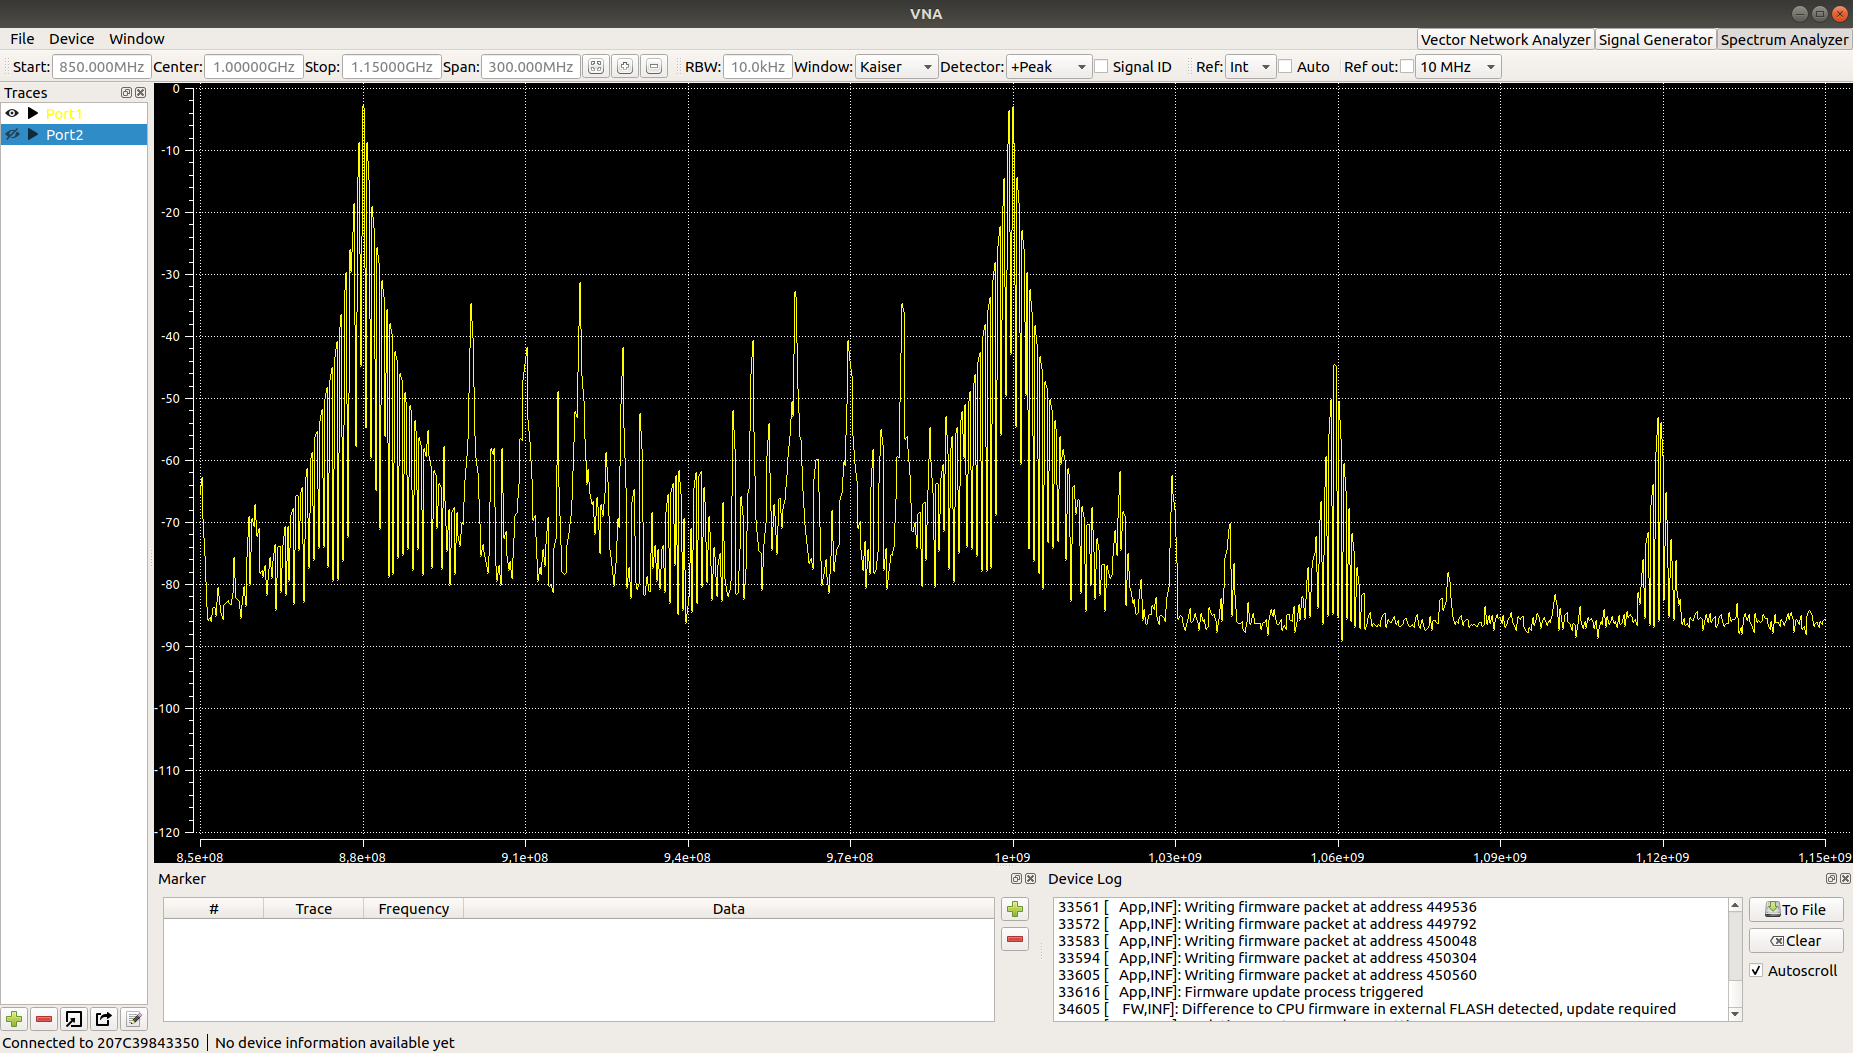
\includegraphics[width=0.48\textwidth]{Screenshots/SASignalIDOff.png}
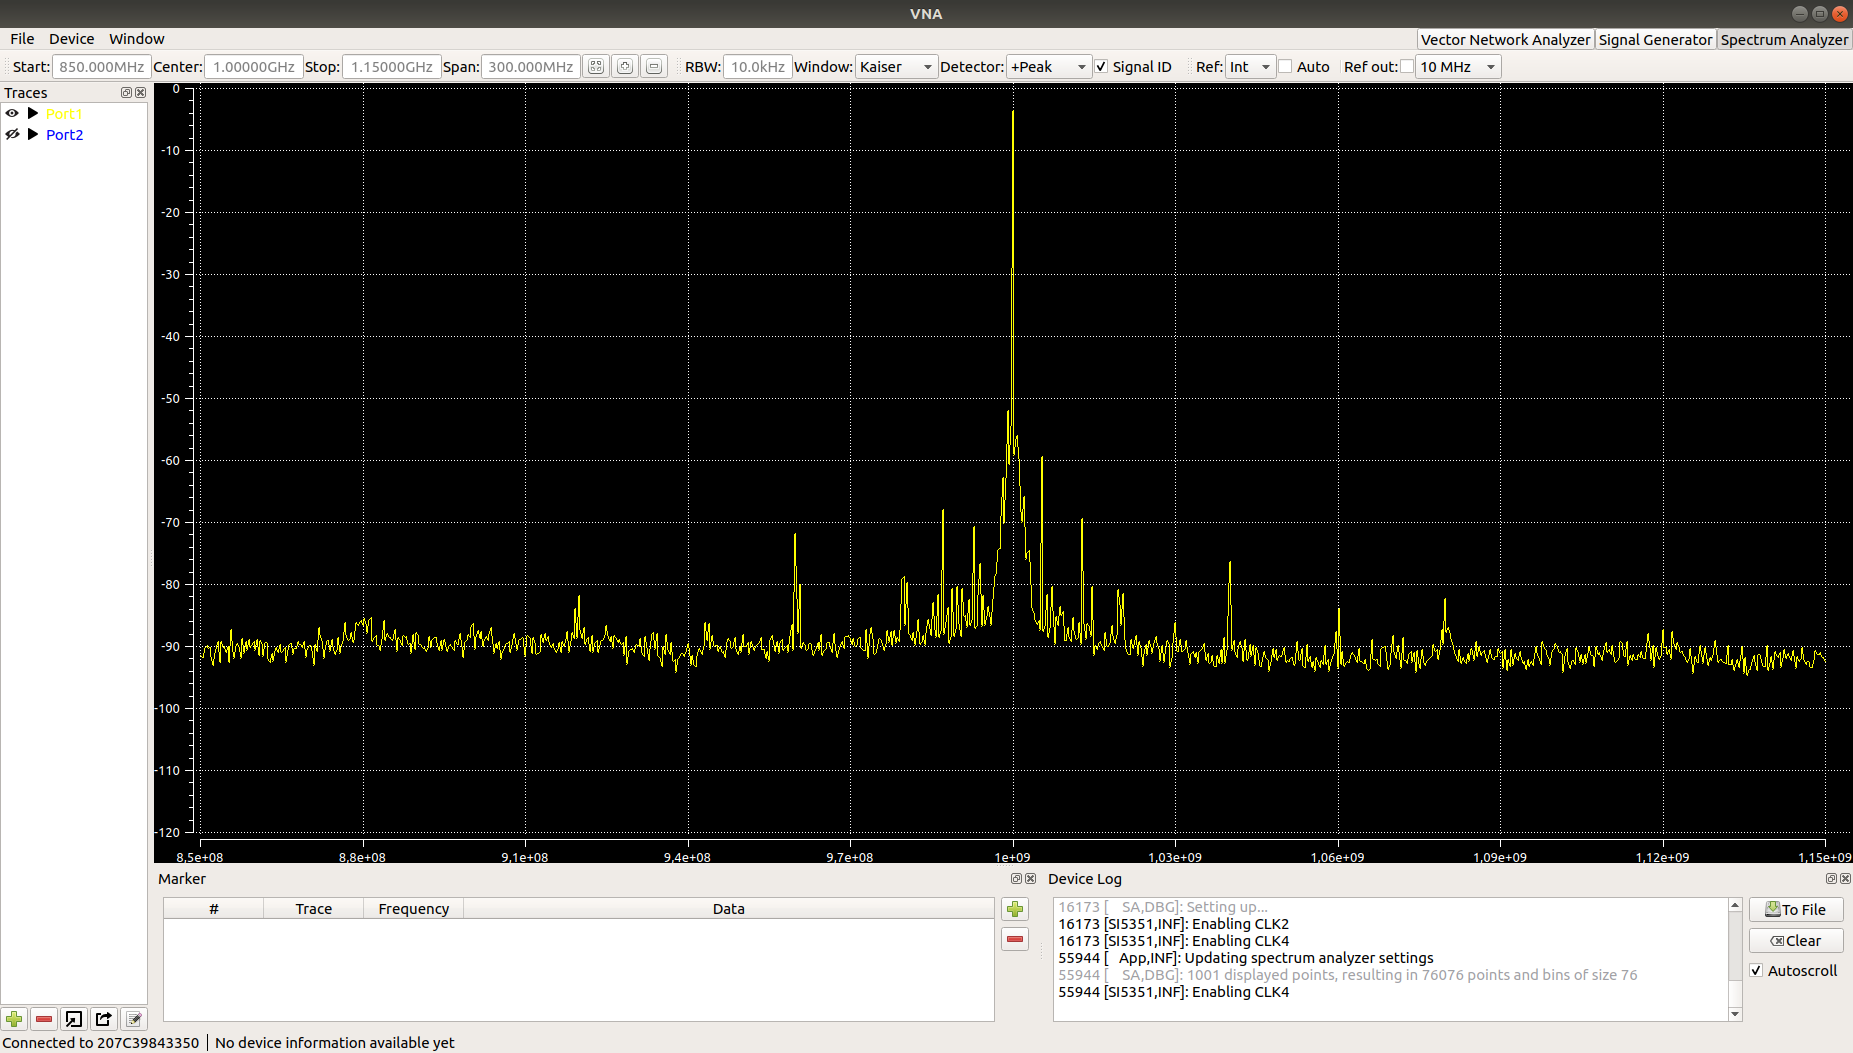
\includegraphics[width=0.48\textwidth]{Screenshots/SASignalIDOn.png}
\end{center}
\end{itemize}

\subsection{Tracking Generator Toolbar}
\screenshot{0.8}{ToolbarTrackingGenerator.png}
A tracking generator at either port is available in the spectum analyzer. If the tracking generator is active at a port, measurements from that port are still available but meaningless. The tracking generator also includes an optional frequency offset. To get accurate results, a Source/Receiver Calibration (section~\ref{amplitude:calibration}) should have been performed when using the tracking generator.

DFT acquisition is not available when the tracking generator is active. Also, due to hardware limitations, the tracking generator is unable to reach every frequency exactly. For narrow spans this could result in "drops" in the spectrum where the signal of the tracking generator is outside of the RBW filters passband. The frequency resolution is frequency dependent. A warning message appears if this could be a problem with the selected span and stop frequency.

\section{Amplitude Calibration}
\label{amplitude:calibration}
This section is about calibrating the source output level and spectrum analyzer level. It does not affect VNA measurements at all. For the VNA calibration, see section~\ref{vna:calibration}.

Both the internal signal source and the receiver paths used in the generator or spectrum analyzer mode have no means of ensuring accurate amplitudes (as imperfections are removed by the VNA calibration, the hardware is not optimized for absolute amplitude accuracy). In order to improve the accuracy of both the generator and the spectrum analyzer (especially with enabled tracking generator), frequency dependent amplitude calibrations are available. They are permanently stored in the device and are only required to be performed once. The \textbf{Source Calibration} corrects the ouput of the (tracking) generator, while the \textbf{Receiver Calibration} corrects the measurement of the spectrum analyzer.

For both calibrations, other test equipment is required, ideally covering the whole range of \SI{1}{\mega\hertz} to \SI{6}{\giga\hertz} (a calibration of only the partial frequeny range is also possible but signals/measurements outside the calibrated range will be inaccurate). The Soure Calibration requires a way to measure the output of the \vna{} (e.g. a spectrum analyzer or power meter), the Receiver Calibration requires a signal source (e.g. a signal generator). Once either calibration has been completed, the \vna{} can also infer the other one with reasonable accuracy.

\subsection{Source Calibration}
Select \menu[,]{Device,Source Calibration}. A window showing the current source calibration opens:
\screenshot{1.0}{SourceCalibration.png}
These are the necessary steps:
\begin{enumerate}
\item \textbf{Set up the calibration frequencies:} Add or remove points according to your needs. Ideally, they should be evenly spaced across the range to calibrate, maybe with a slight emphasis on higher frequencies (signal levels generally vary more at higher frequencies). Additionally, it is advisable to set one point at \SI{25}{\mega\hertz} and one just below (at \SI{25}{\mega\hertz} a band is switched, resulting in an amplitude discontinuity). Up to 64 points can be used.
\item \textbf{Select the calibration mode:} Either calibrate both ports separately (best accuracy but more work) or assume that they are identical and use the measurement at one port for both.
\item \textbf{Perform the calibration:} For each frequency and port, select the corresponding cell in the table. The \vna{} will generate a signal at the selected frequency and port with (what it thinks are) \SI{-20}{\dBm}. Use external equipment to determine the actual output level and enter the measured value into the selected cell.
\item \textbf{Save the calibration:} Once all measurements have been taken, the "Save to Device" button becomes available. There is no way to save intermediate results, you have to calibrate all frequencies you have chosen in step 1.
\end{enumerate}
If the Receiver Calibration is already done, it is also possible to infer the Source Calibration from that. Press \keys{Automatic measurement} and connect both ports of the \vna{} directly to each other. This connection should be as ideal as possible (short, low loss cable) as every imperfection directly translates into calibration errors. During the automatic calibration, the \vna{} uses the already established frequency points from the Receiver Calibration and measures the output amplitude by itself to determine the coefficients of the Source Calibration.
\subsection{Receiver Calibration}
Select \menu[,]{Device,Receiver Calibration}. The Receiver Calibration works almost identically to the Source Calibration. The only difference is in step 3:
\begin{enumerate}
\setcounter{enumi}{2}
\item \textbf{Perform the calibration:} For each frequency and port, select the corresponding cell in the table and apply a signal with known level at the selected frequency and port. The signal level should be in the range of \SI{-40}{\dBm} to \SI{-10}{\dBm}. Higher signal levels might already compress in the receiver while lower levels unnecessary increase calibration errors due to noise. The \vna{} tunes its receiver to the selected frequency and measures the amplitude. Apply the signal for at least \SI{2}{\second} and enter its actual amplitude into the selected cell while the signal is still active.
\end{enumerate}
\section{Troubleshooting}
\label{troubleshooting}
If there was an error in the boot process, the "Booting" LED will blink an error code repeatedly:
\begin{center}
\begin{threeparttable}
\begin{tabularx}{\textwidth}{L{1cm}|X|L{7cm}}
    \toprule
    \textbf{Error Code} & \textbf{Meaning} & \textbf{Possible solution}\\
     \hline
      1   	&      Failed to detect FLASH memory  & Hardware failure, check soldering\\
    \hline
      2   	&      Invalid FLASH content  & Perform firmware update\\
    \hline
      3   	&      Failed to configure FPGA & Check FPGA bitstream generator settings\\
    \hline
      4   	&      Hardware initialization failed & Verify that FPGA bitstream and uC firmware are created from the same release\\
      \bottomrule
\end{tabularx}
\end{threeparttable}
\end{center}
\end{document}
